\documentclass[../main.tex]{subfiles}

\begin{document}

\chapter{Transcriptomic analysis of plasmodesmatal response to fungal chitin}
\label{cha:transcripts}


\begin{figure}[ht]
  \centering
  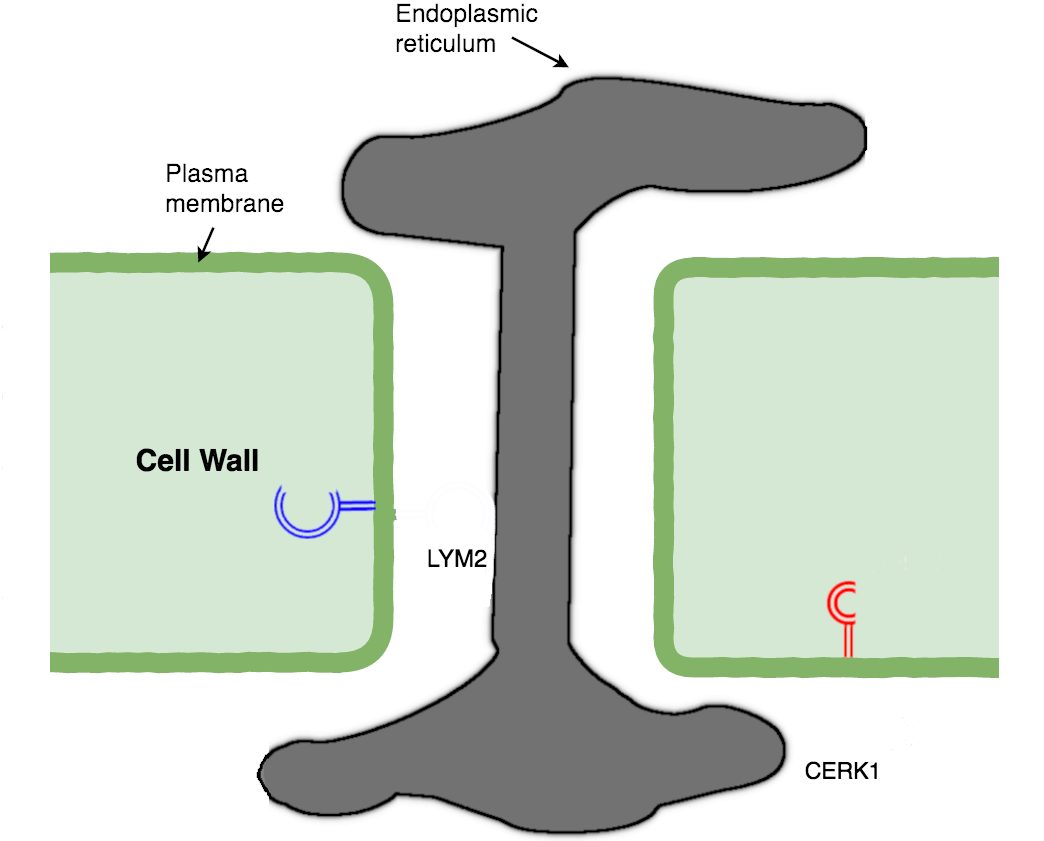
\includegraphics[width=0.5\columnwidth]{figures/original desmotubule.png}
  \caption{\label{fig:receptors} receptor fig}
\end{figure}



\begin{figure}[ht]
  \centering
  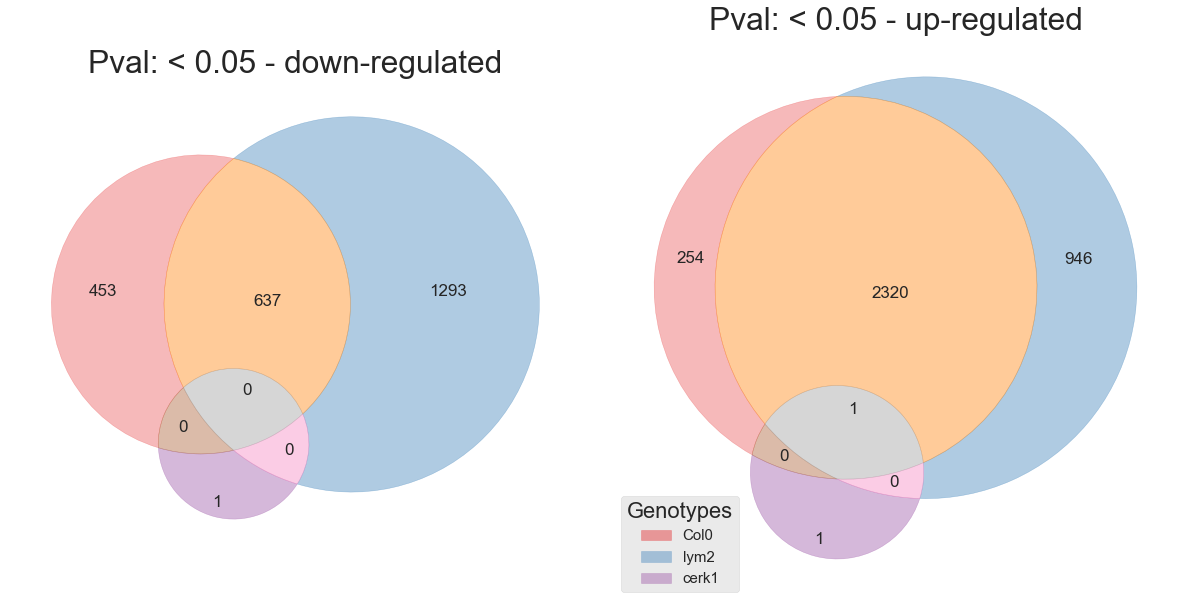
\includegraphics[width=\columnwidth]{figures/vennTreatmentschitin.png}
  \caption{\label{fig:05hrDEGs} DEGs for 05hr}
\end{figure}



\begin{figure}[ht]
  \centering
  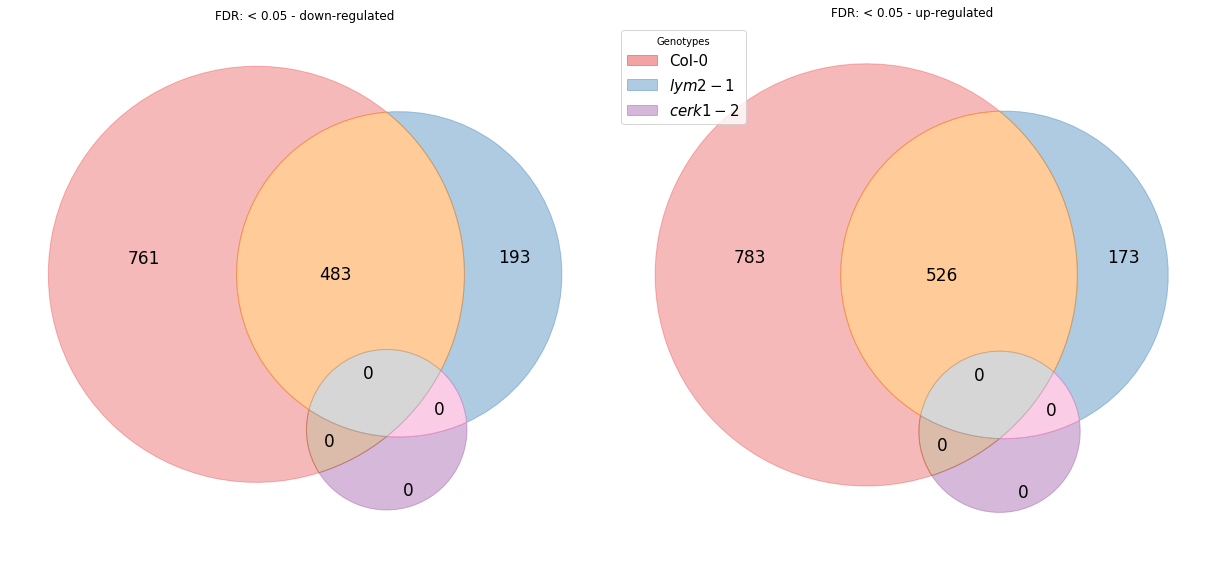
\includegraphics[width=\columnwidth]{figures/vennTreatmentschitin6.png}
  \caption{\label{fig:6hrDEGs} DEGs for 6hr}
\end{figure}


\begin{figure}[!ht]
  \centering
  \subfloat[First sub-figure\label{subfig-1:deg5}]{%
    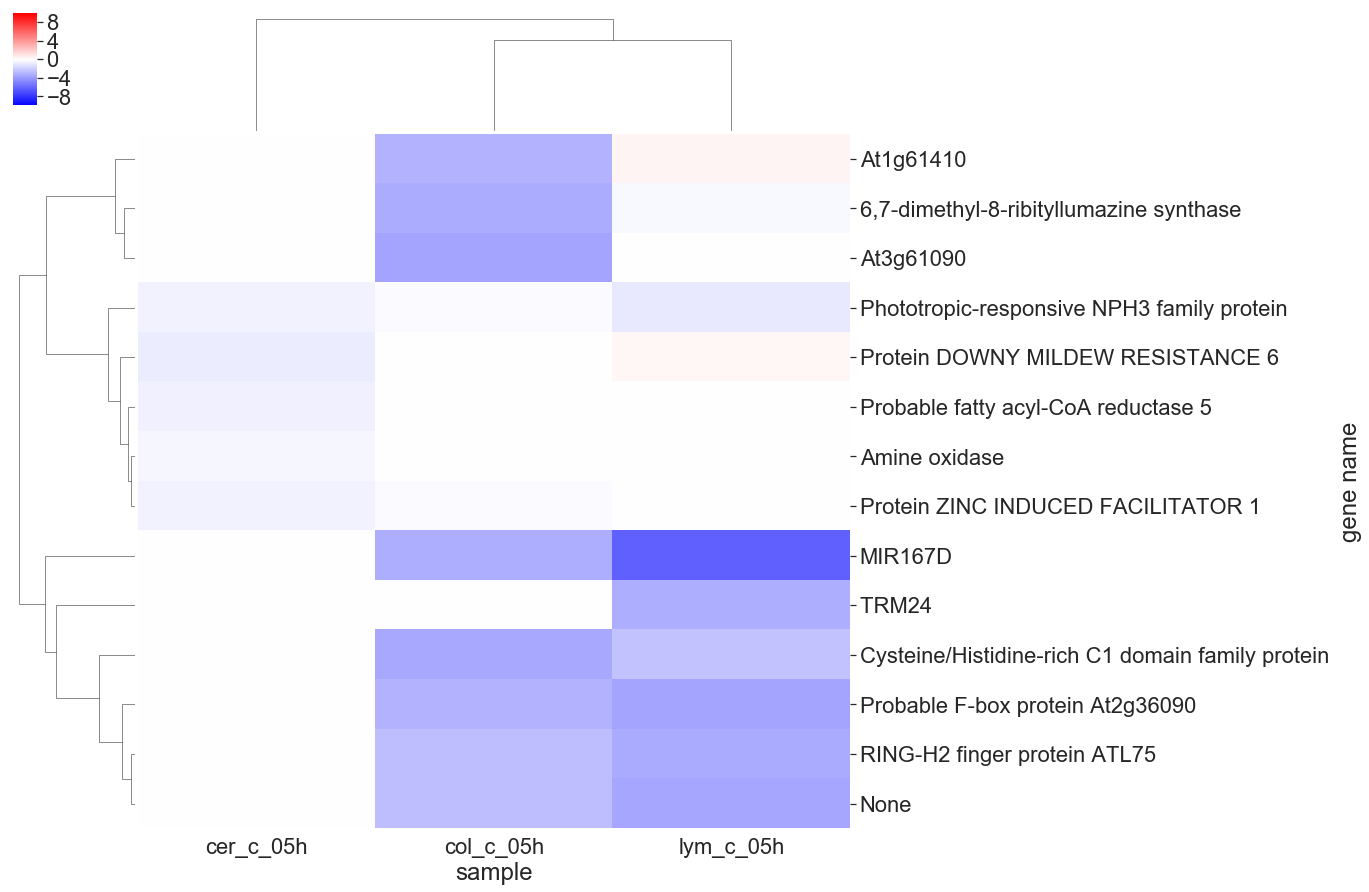
\includegraphics[width=0.7\columnwidth]{./figures/chitin_water_05hr_down.png}
  }
  \\
  \subfloat[First sub-figure\label{subfig-2:deg5}]{%
    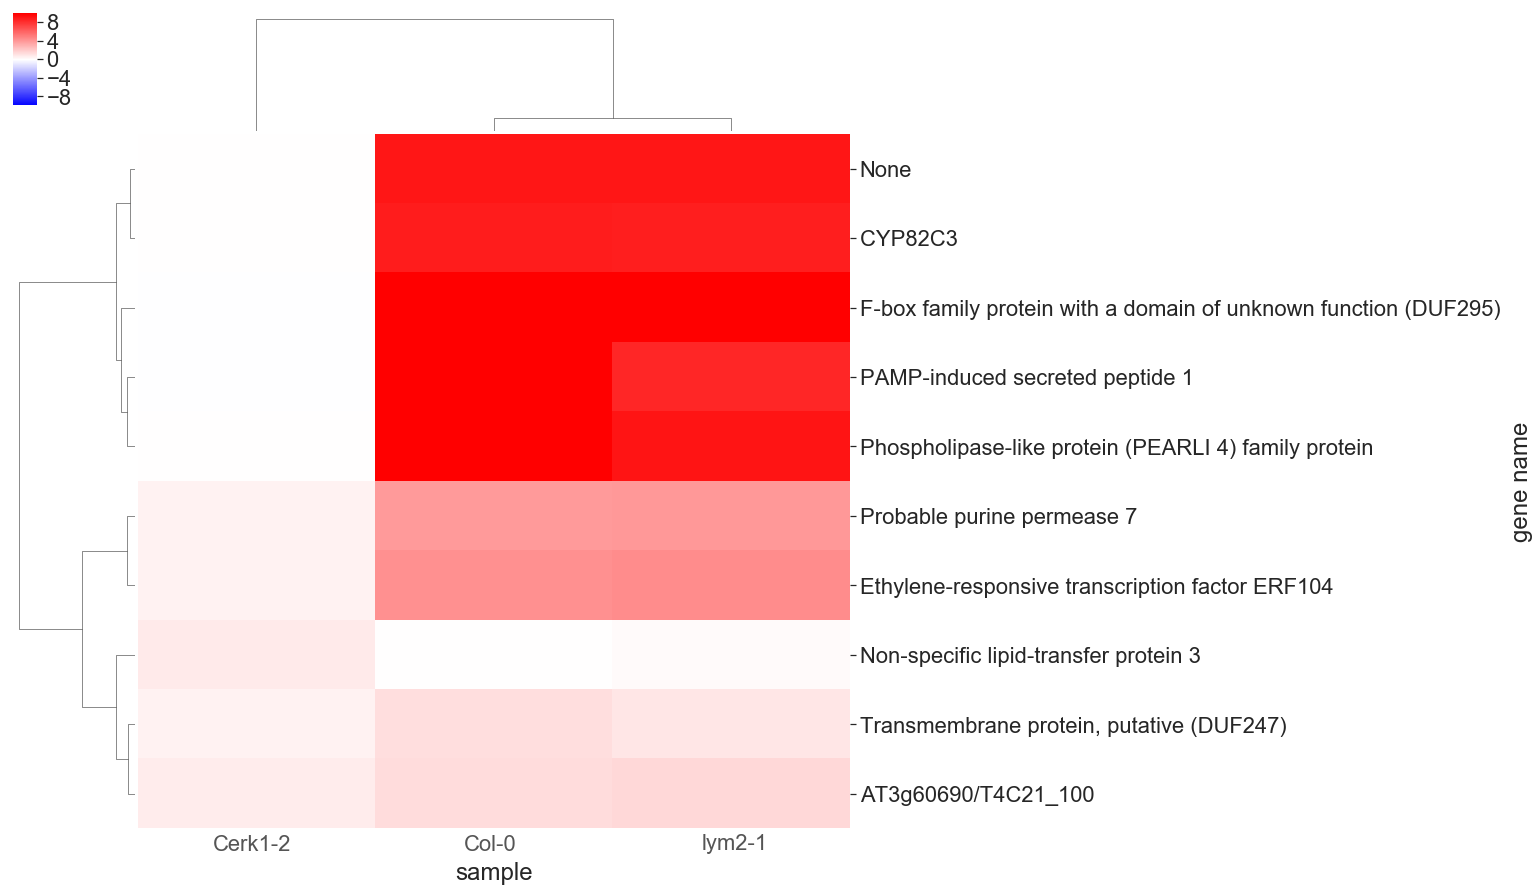
\includegraphics[width=0.7\columnwidth]{./figures/chitin_water_05hr_up.png}
  }
  \caption{DEGs}
  \label{fig:DEG5}
\end{figure}




\begin{figure}[!ht]
  \subfloat[First sub-figure\label{subfig-1:cerk}]{%
    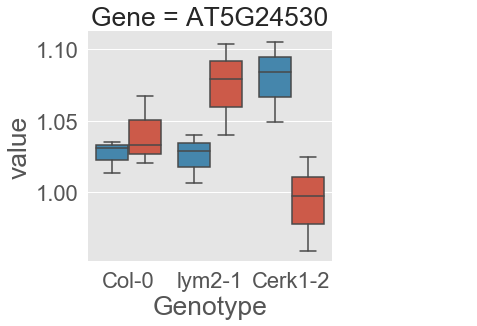
\includegraphics[width=0.5\columnwidth]{./figures/cerk_genes_AT5G24530.png}
  }
  \subfloat[First sub-figure\label{subfig-2:cerk}]{%
    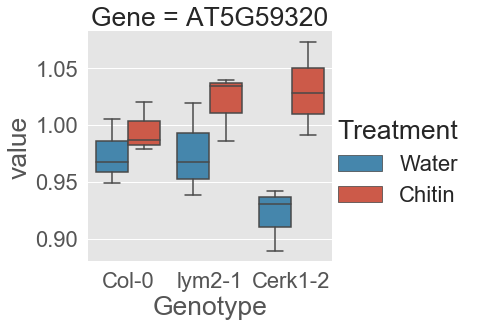
\includegraphics[width=0.5\columnwidth]{./figures/cerk_genes_AT5G59320.png}
  }\\
  \subfloat[First sub-figure\label{subfig-3:cerk}]{%
    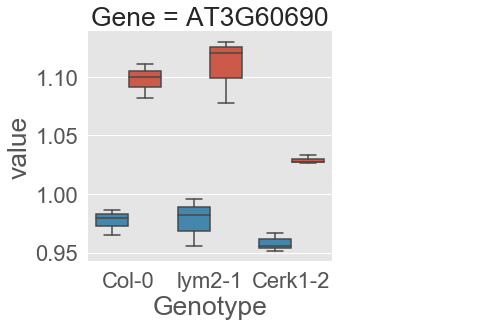
\includegraphics[width=0.5\columnwidth]{./figures/cerk_genes_AT3G60690.png}
  }
  
  \caption{cerk genes}
  \label{fig:cerk}
\end{figure}





\begin{figure}[!ht]
  \centering
  \subfloat[First sub-figure\label{subfig-1:deg6}]{%
    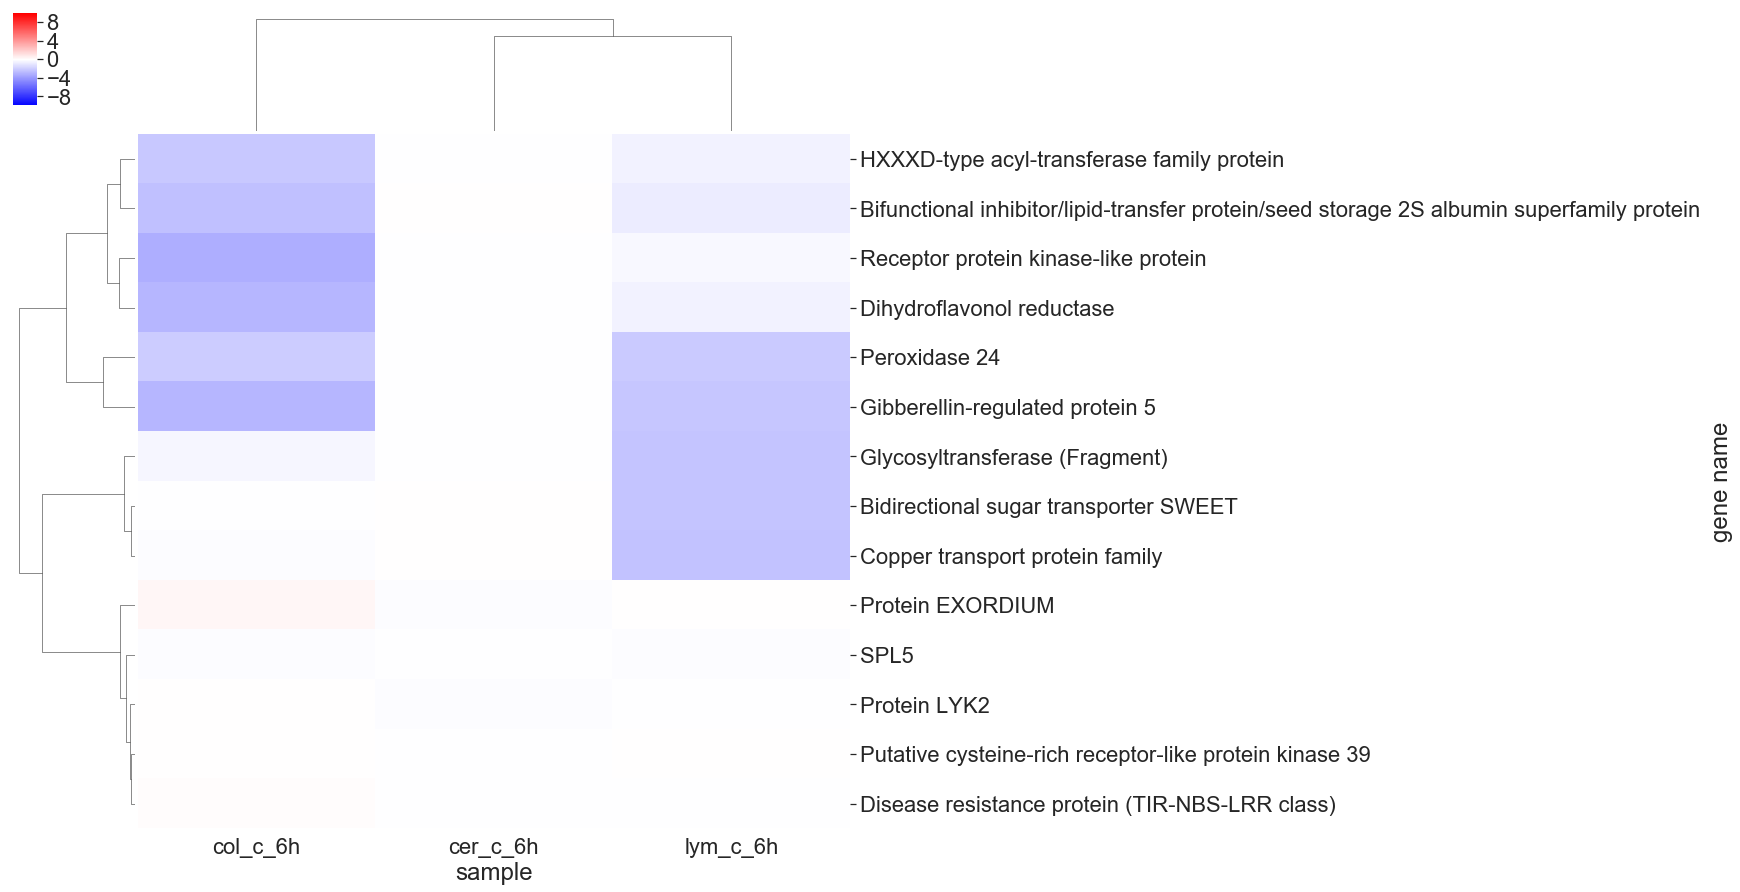
\includegraphics[width=0.7\columnwidth]{./figures/chitin_water_6hr_down.png}
  }
  \\
  \subfloat[First sub-figure\label{subfig-2:deg6}]{%
    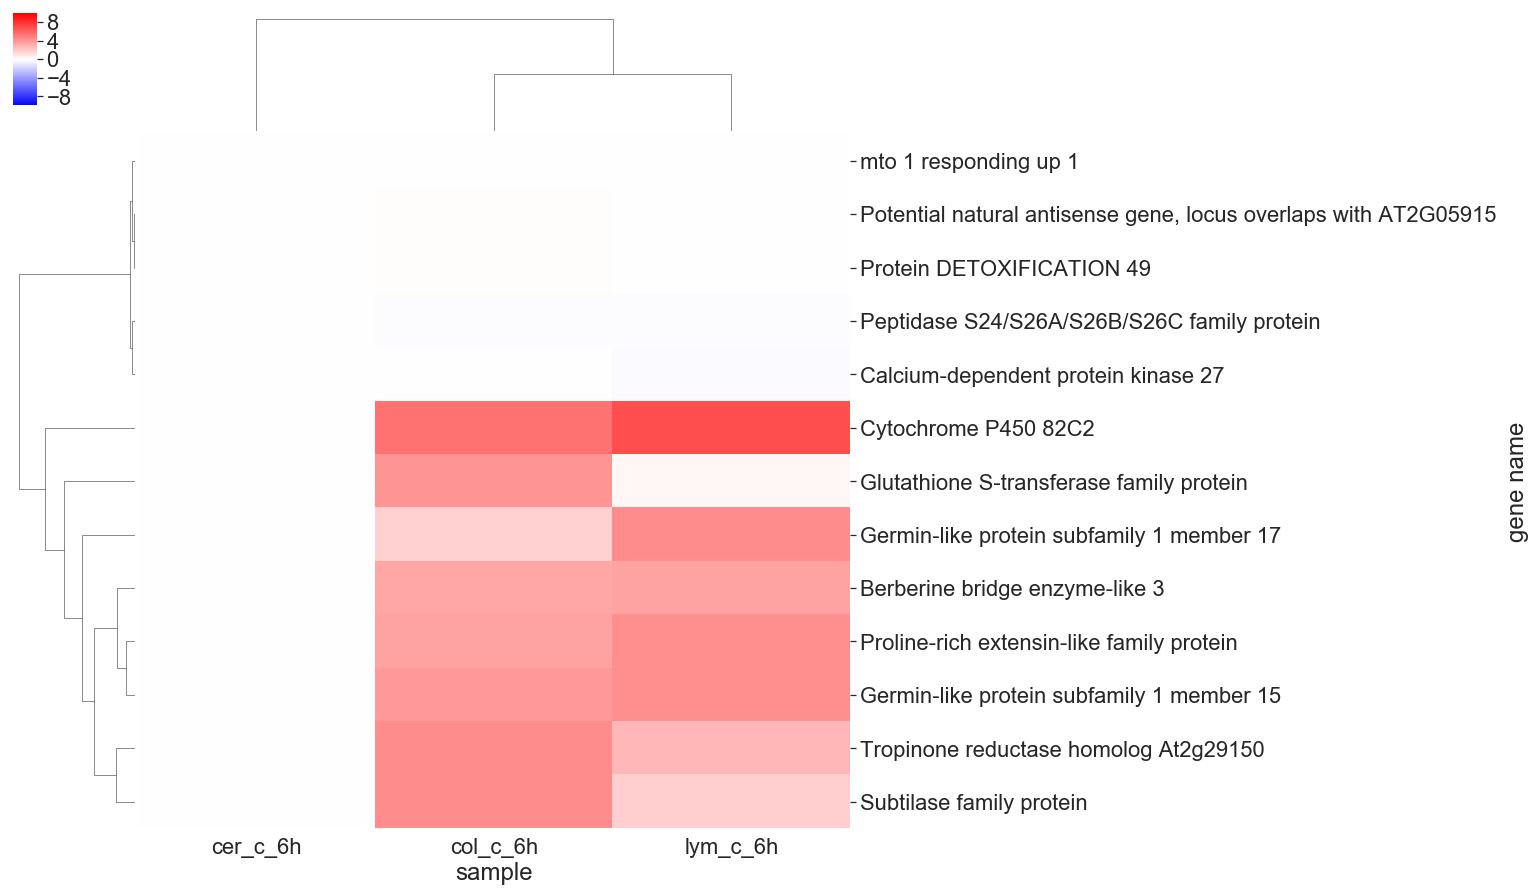
\includegraphics[width=0.7\columnwidth]{./figures/chitin_water_6hr_up.png}
  }
  \caption{DEGs}
  \label{fig:DEG6}
\end{figure}



% trim={5cm 0 0 0},clip


\begin{figure}[ht]
  \centering
  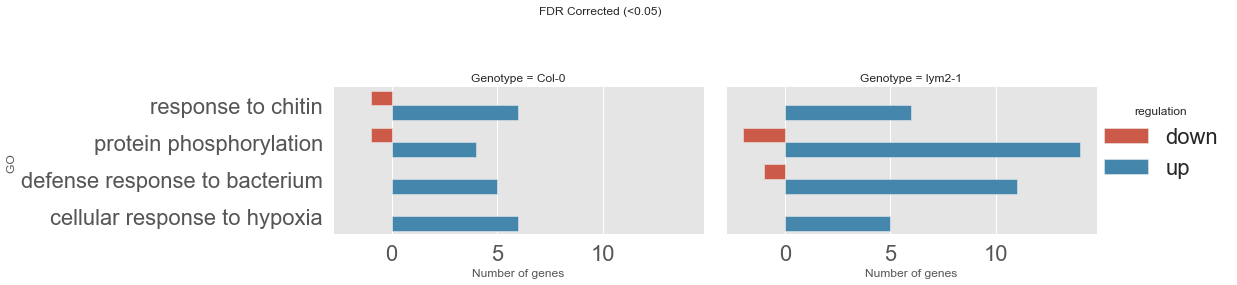
\includegraphics[width=\columnwidth]{figures/05hrGO.png}
  \caption{\label{fig:05hrGO} GO terms for 05hr}
\end{figure}



\begin{figure}[ht]
  \centering
  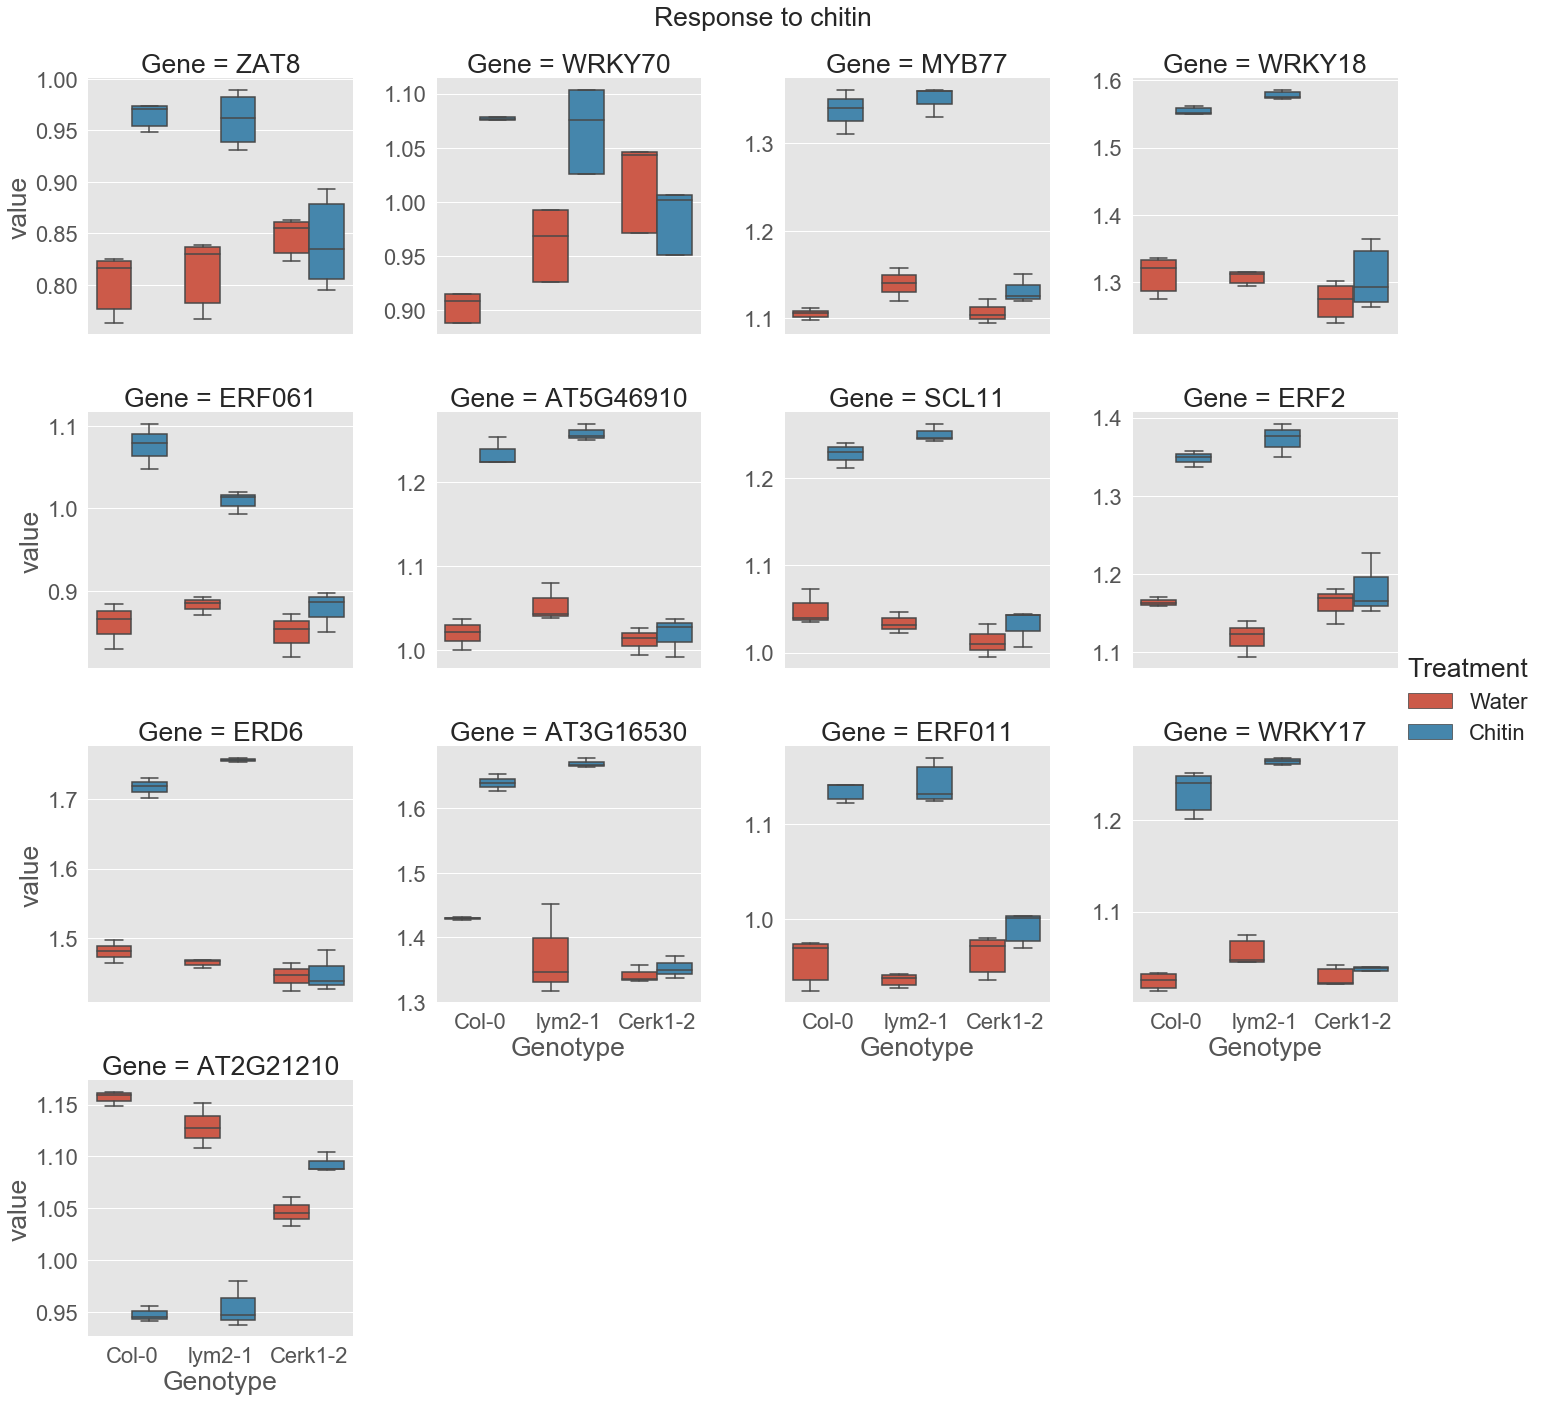
\includegraphics[width=\textwidth, height=\textheight, keepaspectratio]{figures/response to chitin.png}
  \caption{\label{fig:respchitin} Response to chitin genes}
\end{figure}



\end{document}


%%% Local Variables:
%%% mode: latex
%%% TeX-master: "../main"
%%% End:
